\documentclass[11pt,a4paper]{article}
\usepackage[top=3cm, bottom=2cm, left=3cm, right=2cm]{geometry}
\usepackage[utf8]{inputenc}
% \usepackage[T1]{fontenc}
\usepackage{amsmath, amsfonts, amssymb}
\usepackage[brazil]{babel}
\usepackage{graphicx}
\usepackage[margin=10pt,font=small,labelfont=bf]{caption}
\usepackage[dvipsnames, svgnames]{xcolor}
\DeclareCaptionFont{MediumOrchid}{\color[svgnames]{MediumOrchid}}
\usepackage[pdftex]{hyperref}
\usepackage{natbib}
\bibliographystyle{plainnat}
\bibpunct{[}{]}{,}{s}{}{}
\usepackage{color}
\usepackage{footnote}
\usepackage{setspace}
\usepackage{booktabs}
\usepackage{multirow}
\usepackage{fancyhdr}
\usepackage{leading}
\usepackage{indentfirst}
\usepackage{wrapfig}
\usepackage{float}
\renewcommand{\thefootnote}{\alph{footnote}}
\usepackage{url}
\hypersetup{
    colorlinks=true,
    linkcolor=cyan,
    filecolor=cyan,      
    urlcolor=cyan,
    citecolor=cyan,
    pdftitle={Braquiterapia}
}
\pagestyle{fancy}
\fancyhf{}
\renewcommand{\headrulewidth}{0pt}
\rfoot{Página \thepage}
\title{Braquiterapia}
\author{Tratamentos por Sítio Anatômico\nocite{*}}
\date{\textit{Dalila Mendonça}}
\begin{document}
	\maketitle

    \section{Braquiterapia Oftalmológica}

% Introdução:
% É utilizada no tratamento de Melanomas Oculares/Coroidais e em Retinoblastoma, este sendo mais comum em pacientes neonatais e bebês.. Os tratamentos possíveis para estas doenças são a enucleação (retirada do olho) ou a braquiterapia com placas oftalmicas. Iniciou-se com o Co - 60 e subsequentemente foram tentados iridio 192, rutenio 106, iodo 125  paladio 103 estroncio 90 e césio 131. Antes de 2002 os guidelines eram focados no i 125 mas conforme a utilização de outras fontes, novos protocolos foram estabelecidos pela American Brachyterapy Society. Collaborative Ocular Melanoma Study (COMS) é um ensaio clinico multi disciplinar que desenvolveu estudos randomizados e padronizou métodos de placas de braquiterapia para melanomas coroidais.


% Critério de Exclusão: 
% Tumores com extensão extraoculares grosseiros (T4e ou maior de 5cm), diâmetros basais que excedem os limites de braquiterapia e olho doloroso cego e sem percepção de luz.

% Possíveis reações: 
% Efeitos tardios - predominantes: Retinopatia radio-induzida, catarata, necrose escleral, Vazamento vascular periférico da retina com exsudação e hemorragia.
% Tumores próximos a fovea e ao nervo ótico pode causar morbidades como a cegueira. Quanto maior a distância entre a placa e a mácula ou o nervo ótico melhor o resultado visual. É possivel evitar a incidendia de retinopatoa por radiação e neuropatia ótica apliocando injeções intravítras de triancinolona e agentes anti-fator de crescimento endotelial vascular.

% Planejamento de Tratamento: 
% É necessário informações do oftamologista quanto a lateralidade, estágio, tamanho do tumor (diâmetro e altura) que devem ser confirmados através de uma ultrassom e um diagrama de fundo detalhado contendo a localização do tumor, medidas tumorais assim como a distância do tumor até a fóvea, nervo ótico, glandula lacrimal,  cristalino e o olho oposto. os dados do diagrama de fundo são transferidos para o TPS, é inserido os dados dosimétricos da fonte de radiação escolhida para o procedimento e então a dose no tumor e a dose nos OAR são calculadas com base na COMS e no TG-129

%   - Diametros do tumor devem ser menores que o PTV ou o diâmetro da placa para evitar perca geografica.
%   - O ponto de prescrição deve ser no ápice do tumor, que é o ponto de espessura máxima.
%   - A isodose de prescrição deve cobrir todo o tumor para maximizar o controle local
%   - A prescrição de dose para o Retinoblastoma é de 40Gy a 45Gy ente 1 - 5 dias
%   - A dose total no ápice tumoral pode variar dependendo do radionuclídio escolhido, entre 70Gy a 100Gy.
%   - A prescrição de Dose comum para o Melanoma Coroide é de 85Gy em um mínimo de 5mm de profundidade utilizando uma placa com 0.2 cm de margem em torno do diâmetro basal do tumor, que deve ser entregue entre 3 - 7 dias consecutivos. .
%   -  Esta prescrição em um meio homogênio entrega 75Gy a 5mm de profundidade para o I-125 e 69Gy a 5mm de profundidade para o Pd-103
%   - Existe um gradiente de dose e portanto a dose máxima pode variar com a profundidade de tratamento e dependendo do Radionuclídio utilizado. 
%   - I-125: 85Gy, 10 mm dmax (inner-scleral)  644 Gy, 3 mm dmax = 166 Gy, 5mm dmax  = 260
%   - Emissores Beta (Ru-106 e Rh 106), 5mm dmax = 800 Gy, são indicados para tratar lesões com espessura do ápice menor que 5 - 6 mm
%   - As placas de 106-Ru são finas, em torno de 1 mm
%   - Pd 21Kev, I125 28Kev e Cs 131 30Kev : aumenta progressivamente o gradiente de dose do menor para o maior; Aumenta a dose na esclera e diminui nas estruturas oculares normais.
%   - Métodos de calculos heterogêneos acarretam em uma diferença de dose superior a 10\% 
%   - A taxa de dose não deve ser menor que o padrão COMS equivalente de 0.60Gy/h para o I/125
%   - A atividade típica de I125 utilizada por semente varia entre 0.5 - 5mCi para alcançar tazas de dose ente 0.5 - 1.25Gy/h 
%   - A lçocalização do tumor pode ser feita utilizando fundoscopia, fotografia  de fundo e ultrassom. CT e RM pode ser utilizada. Pós implante a verificação da posição das placas é feita com ultrassom.
%   - Além das fontes já citadas, podem ser utilizadas Sr-90/Y-90 (emissores beta), e Co-60 



% Cirurgia:
% Recomenda-se uma equipe multidisciplinar de oncologista oftamologico, radio oncologista e físico médico. O tumor é localizado pelo cirurgião e é medido para identificar qual diâmetro de placa será utilizado, que deve considerar o diâmetro do tumor e a margem de planejamento. Na sequência a placa ocular é afixada na esclera ( tecido fibroso que reveste o olho) através de suturas e caso algum musculo ocular esteja impedindo a inserção da placa ele é realocado. O tempo de inserção é registrado do registro de radiação e um tapa olho de chumbo é colocado sobre o olho afetado. Em seguida a placa permanece no local durante todo o tempo pré-planejado para fornecer a dose apropriada na profundidadee em seguida a placa é removida sob anestesia local e qualquer músculo ocular que tenha sido realocado para conseguir inserir a placa é colocado em seu lugar novamente



% TODO: wrapfigure tá gata
 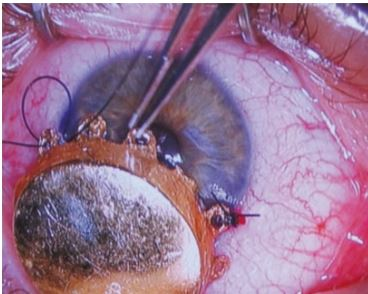
\includegraphics{Imagens/placaComsOuroMC.JPG}
 % \caption{Fotografia externa da placa COMS feita de uma liga de ouro, costurada na esclera após a localização}

 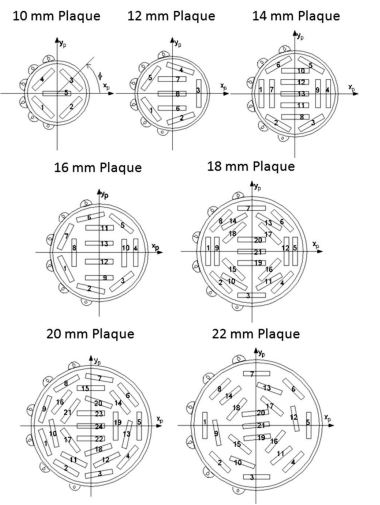
\includegraphics{Imagens/placasComs.JPG}
 % \caption{Diagrama das sementes distribuidas em placas COMS. Consistem em um suporte feito de uma liga de ouro com um portador de sementes feitos de Silastic(borracha de silicone) acoplados no suporte.}

 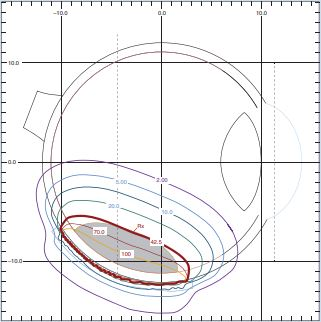
\includegraphics{Imagens/distribDosePlacaOftamRutenio.JPG}
 % \caption{Distribuição de Isodose para uma Placa de Rutênio de 15.3mm modelo CCA, o alvo é a sombra cinza. Devido ao acentuado falloff de dose a profundidade de tratamento dessas placas são limitadas a5-6mm a partir da superfície da placa.}

 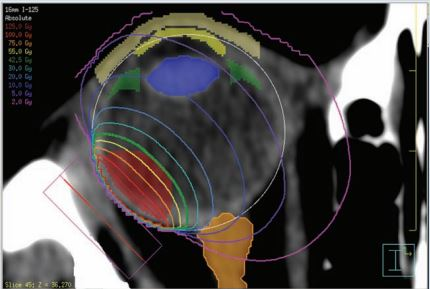
\includegraphics{Imagens/distribDosePlacaComsI125.JPG}
 % \caption{Corte axial de TC mostrando a distribuição de isodose para uma placa de I125 COMS de 16mm para entregar 42.5Gy no alvo (em vermelho). O perfil de dose baseado em Monte-Carlo, que considera os efeitos da capa de outro e a atenuação nos portadores de silicone, foi atribuído a fonte, representada pelo retângulo. }
% TODO: pegar dados no TG 129 e no guideline da ABS

    \section{Braquiterapia de Cabeça e Pescoço}



    \section{Braquiterapia de Mama}

    \section{Braquiterapia Toráxica}

    \section{Braquiterapia de Fígado}

    \section{Braquiterapia Ginecológica}
    
    \section{Braquiterapia de Próstata}

    \section{Braquiterapia Gastrointestinal}

    \section{Braquiterapia Superficial}

    \section{Braquiterapia Intravascular}



\bibliography{ref.bib}
\end{document}
